% =====================================================================
%  Diapositivas — Efecto Mpemba cuántico en HPC
%  Charla conjunta Juan (teal) / Sebastián (naranja). 16:9, ~12-15 min.
%  Compilar DESDE esta carpeta:
%    pdflatex diapositivas_qmpe && bibtex diapositivas_qmpe && pdflatex x2
% =====================================================================
\documentclass[aspectratio=169,10pt]{beamer}
\usepackage[utf8]{inputenc}
\usepackage[T1]{fontenc}
\usepackage[spanish,es-noshorthands]{babel}
\usepackage{amsmath,amssymb,bm}
\usepackage{graphicx,booktabs}
\usepackage{xcolor}
\usepackage{listings}
\graphicspath{{../}}

\usetheme{default}
\setbeamertemplate{navigation symbols}{}
\setbeamertemplate{footline}[frame number]
\setbeamertemplate{itemize items}[circle]

% ---- paleta y autores ----
\definecolor{juan}{RGB}{15,115,140}     % Juan = teal
\definecolor{seb}{RGB}{205,95,25}       % Sebastián = naranja
\definecolor{ink}{RGB}{33,37,48}
\definecolor{soft}{RGB}{120,125,135}
\setbeamercolor{frametitle}{fg=ink}
\setbeamercolor{title}{fg=ink}
\setbeamercolor{structure}{fg=ink}
\setbeamercolor{normal text}{fg=ink}
\setbeamerfont{frametitle}{series=\bfseries}

\newcommand{\J}{\hfill\colorbox{juan}{\color{white}\scriptsize\bfseries~Juan~}}
\newcommand{\Sb}{\hfill\colorbox{seb}{\color{white}\scriptsize\bfseries~Sebastián~}}
\newcommand{\cj}[1]{\textcolor{juan}{\textbf{#1}}}
\newcommand{\cs}[1]{\textcolor{seb}{\textbf{#1}}}
\newcommand{\rss}{\rho_{\mathrm{ss}}}
\newcommand{\Lop}{\mathcal{L}}
\newcommand{\ket}[1]{\lvert #1\rangle}
\newcommand{\bra}[1]{\langle #1\rvert}
\newcommand{\dyad}[2]{\lvert #1\rangle\langle #2\rvert}

% ---- estilo de código ----
\lstdefinestyle{core}{
  basicstyle=\ttfamily\scriptsize,
  keywordstyle=\color{blue!55!black}\bfseries,
  commentstyle=\color{green!40!black}\itshape,
  stringstyle=\color{red!55!black},
  emph={pragma,omp,parallel,for,schedule,MPI_Reduce,MPI_Allgatherv,MPI_Init,
        executor,map,ThreadPoolExecutor},
  emphstyle=\color{seb}\bfseries,
  showstringspaces=false, columns=fullflexible, breaklines=true,
  keepspaces=true, tabsize=2,
}
\lstset{style=core}

% ---- cabecera de sección coloreada por autor ----
\newcommand{\divider}[3]{% color, autor, titulo
  \begingroup
  \setbeamercolor{background canvas}{bg=#1}
  \begin{frame}[plain]
    \vfill
    \begin{center}
      {\color{white}\Large\bfseries #3}\\[4pt]
      {\color{white!85}\small #2}
    \end{center}
    \vfill
  \end{frame}
  \endgroup}

\title{\bfseries El efecto Mpemba cuántico en HPC}
\subtitle{Modos lentos, evolución temporal, trayectorias y redes tensoriales}
\author{\cj{Juan} \quad\textbar\quad \cs{Sebastián}}
\institute{\small Sistemas Distribuidos / HPC --- 2026}
\date{}

\begin{document}

% ---------------------------------------------------------------- TÍTULO
{\setbeamertemplate{footline}{}
\begin{frame}[plain]
  \titlepage
  \begin{center}\small
    \textcolor{soft}{Implementación serial y paralela (OpenMP · MPI · CUDA), con validación y escalado}
  \end{center}
\end{frame}}

% ---------------------------------------------------------------- AGENDA
\begin{frame}{Hoja de ruta}
  \begin{columns}[T]
  \begin{column}{0.5\textwidth}
    \begin{enumerate}[1.]
      \item \cj{De lo clásico (macro) a lo cuántico}
      \item \cj{T1 — Modos lentos del Liouvilliano}
      \item \cs{Evolución temporal (a): RK4 directo}
      \item \cs{Evolución temporal (b): Krylov}
    \end{enumerate}
  \end{column}
  \begin{column}{0.5\textwidth}
    \begin{enumerate}[1.]\setcounter{enumi}{4}
      \item \cs{Muchos cuerpos: trayectorias (MPI)}
      \item \cj{Muchos cuerpos: redes tensoriales}
      \item \cj{Conclusiones generales}
      \item \cs{Relevancia en el efecto macro/meso}
    \end{enumerate}
  \end{column}
  \end{columns}
  \vfill
  \begin{center}\small\textcolor{soft}{%
    \colorbox{juan}{\color{white}~Juan~} modos lentos · redes tensoriales \quad
    \colorbox{seb}{\color{white}~Sebastián~} evolución temporal · trayectorias · GPU}
  \end{center}
\end{frame}

% ====================================================================
\divider{juan}{Juan}{1 · De lo clásico a lo cuántico}

\begin{frame}{El efecto Mpemba: una anomalía de relajación\J}
  \begin{columns}[T]
  \begin{column}{0.56\textwidth}
    \small
    \textbf{Clásico (macro).} A veces el agua \emph{más caliente} se congela
    \emph{antes} que la templada: la curva que parte más lejos del equilibrio lo
    alcanza primero \cite{MpembaOsborne1969,LuRaz2017,Kumar2022,Bechhoefer2021}.
    \medskip

    \textbf{Cuántico.} En sistemas abiertos markovianos el fenómeno reaparece como
    un \cs{cruce de las curvas de distancia} al estado estacionario
    \cite{Carollo2021,Nava2024}.
    \medskip

    \textbf{La firma universal:} dos preparaciones, la que parte \emph{lejos}
    \textbf{adelanta} a la que parte \emph{cerca} en un tiempo $t^*$.
  \end{column}
  \begin{column}{0.44\textwidth}
    \centering
    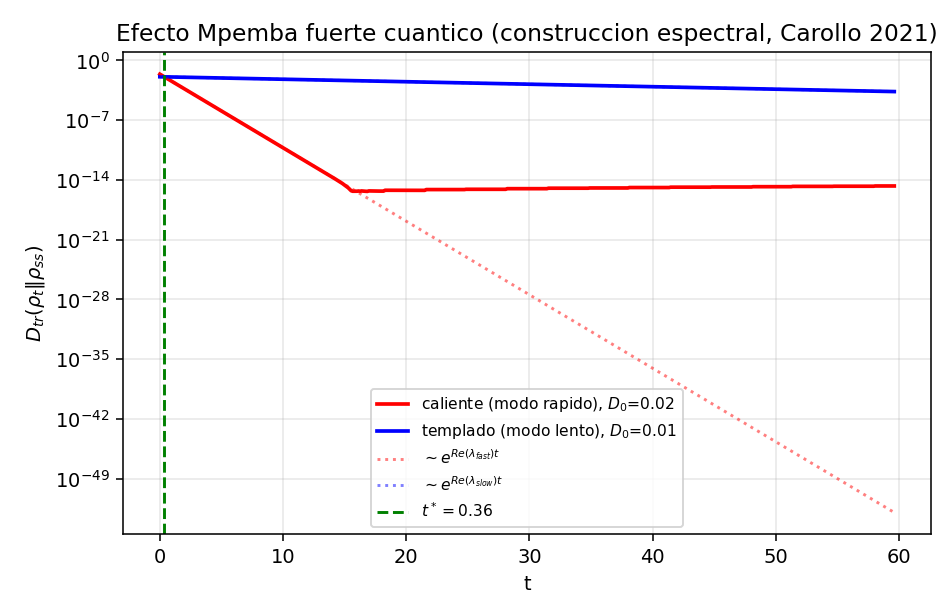
\includegraphics[width=\linewidth]{context/figures/03_mpemba_strong.png}\\
    {\scriptsize\textcolor{soft}{Cruce de curvas: el corazón del efecto.}}
  \end{column}
  \end{columns}
\end{frame}

\begin{frame}{La matemática: ecuación GKSL y autovalores\J}
  \small
  \textbf{Dinámica markoviana (Lindblad / GKSL)} \cite{Lindblad1976,GKS1976,BreuerPetruccione2002}:
  \[
  \dot\rho=\Lop[\rho]=-i[H,\rho]+\sum_\mu\Big(L_\mu\rho L_\mu^\dagger-\tfrac12\{L_\mu^\dagger L_\mu,\rho\}\Big).
  \]
  \textbf{Descomposición espectral del Liouvilliano} (autovalores $\lambda_k$, $\mathrm{Re}\,\lambda_k\le0$):
  \[
  \rho_t=\rss+\sum_{k\ge2}\, a_k\,e^{\lambda_k t}\,\hat r_k,\qquad
  a_k=\mathrm{Tr}(\hat l_k^\dagger\rho_0).
  \]
  \begin{itemize}\small
    \item Relajación dominada por el \cs{modo lento} $\lambda_2$ ($\tau=1/|\mathrm{Re}\,\lambda_2|$).
    \item \cs{Criterio de Mpemba (fuerte)}: si $a_2=\mathrm{Tr}(\hat l_2^\dagger\rho_0)=0$,
      la preparación \emph{salta} el modo lento y relaja a la tasa rápida $\Rightarrow$ cruce \cite{Carollo2021,Chattopadhyay2026}.
    \item No-normalidad de $\Lop$ ($\Lop\Lop^\dagger\!\neq\!\Lop^\dagger\Lop$): los modos no son ortogonales $\Rightarrow$ permite el adelantamiento.
  \end{itemize}
\end{frame}

\begin{frame}{El espectro del Liouvilliano $\Lop$\J}
  \centering
  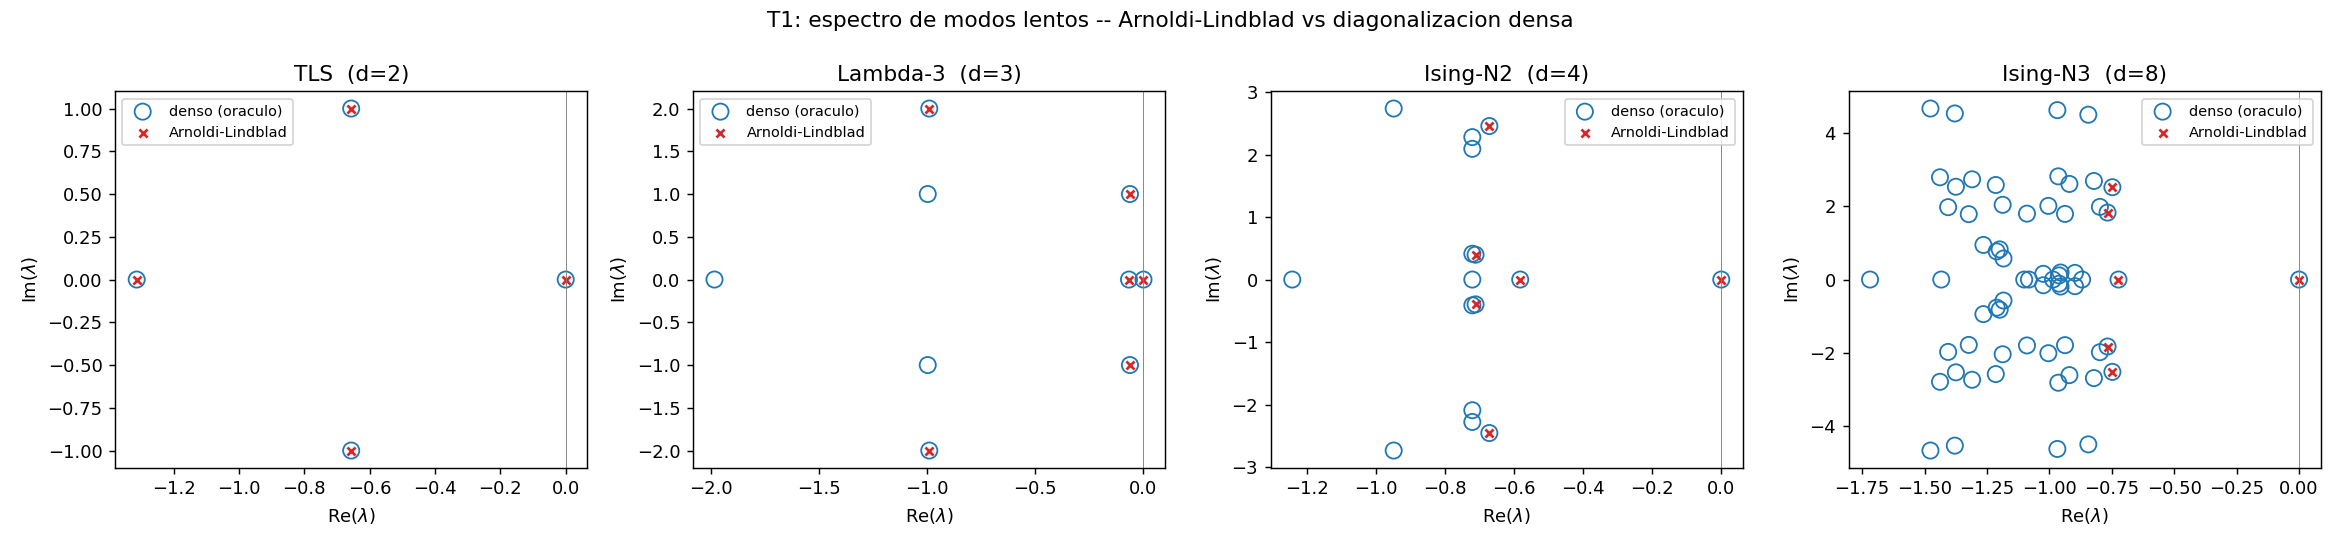
\includegraphics[width=\linewidth]{juan/T1/results/t1_eigs.png}\\[4pt]
  {\small Autovalores $\lambda_k$: $\lambda_1{=}0$ (estacionario $\rss$), todos con
  $\mathrm{Re}\,\lambda_k\le0$. El \cs{modo lento} $\lambda_2$ ---el más cercano a $0$---
  fija la relajación y controla el cruce de Mpemba.}
\end{frame}

\begin{frame}{Predicción del cruce: del espectro, \emph{sin evolucionar}\J}
  \small
  \textbf{Dos preparaciones} (estados producto puros), misma referencia $\rss$ (NESS):
  $\rho_A=\ket{+}^{\otimes N}$ (\cs{parte LEJOS}) y $\rho_B=\ket{0}^{\otimes N}$
  (\cs{parte CERCA}). Con el espectro (T1: $\lambda_2,\hat l_2$) y los solapamientos
  $a_k=\mathrm{Tr}(\hat l_k^\dagger\rho_0)$ \emph{(una traza, sin integrar)}:
  \begin{center}\renewcommand{\arraystretch}{1.05}
  \begin{tabular}{lcc}
  \toprule
  estado & $D_0$ (arranque) & $|a_2|$ (peso modo lento $\lambda_2{=}{-}0.70$) \\
  \midrule
  $\ket{+}^{\otimes N}$ (lejos) & \textbf{0.99} & \textbf{0.13} \\
  $\ket{0}^{\otimes N}$ (cerca) & 0.84 & 0.50 \\
  \bottomrule
  \end{tabular}\end{center}
  \begin{center}\colorbox{seb!12}{\parbox{0.93\textwidth}{\centering\small
  $\ket{+}$ \textbf{arranca más alto} pero \textbf{pesa menos en el modo lento}
  $\Rightarrow$ \cs{cruce garantizado}, $t^*_{\rm pred}\!\approx\!0.68$ ---
  \emph{antes de evolucionar}. T2/T3 lo confirman.}}\end{center}
\end{frame}

% ====================================================================
\divider{juan}{Juan}{2 · T1 — Modos lentos del Liouvilliano}

\begin{frame}{T1 — Método numérico y discretización\J}
  \small
  \textbf{Objetivo.} Extraer los autovalores de $\Lop$ \emph{más cercanos a 0}
  ($\lambda_2,\lambda_3,\dots$) y el solapamiento $a_k$, sin diagonalizar la matriz
  $4^N\times4^N$.
  \medskip

  \textbf{Método: Arnoldi sobre el propagador} $P(\tau)=e^{\tau\Lop}$
  \cite{Minganti2018,Lehoucq1998}.
  \begin{itemize}
    \item Acción \emph{matrix-free} de $P$: se integra $\dot V=\Lop[V]$ con RK4
      (no se forma $\Lop$).
    \item Como $\mu_k=e^{\tau\lambda_k}$ y $\mathrm{Re}\,\lambda_k\le0$, los modos
      \emph{lentos} de $\Lop$ son los \emph{dominantes} de $P$ $\Rightarrow$ Arnoldi
      los extrae primero (\emph{``faster than the clock''}).
  \end{itemize}
  \medskip
  \textbf{Paralelización.} Arnoldi es secuencialmente acoplado $\Rightarrow$ el
  paralelismo vive en el \cs{SpMV} (producto de matrices), no entre iteraciones.
\end{frame}

\begin{frame}[fragile]{T1 — Núcleo: serial \textbar\ paralelo (MPI+OpenMP)\J}
  \begin{columns}[T]
  \begin{column}{0.48\textwidth}
  \centering\textbf{\small Serial}
\begin{lstlisting}[language=C++]
// producto C = A*B
for (int i=0;i<d;++i)
 for (int k=0;k<d;++k){
  cd a=A[i*d+k];
  for (int j=0;j<d;++j)
   C[i*d+j]+=a*B[k*d+j];
 }
\end{lstlisting}
  \end{column}
  \begin{column}{0.52\textwidth}
  \centering\textbf{\small Paralelo (datos)}
\begin{lstlisting}[language=C++]
#pragma omp parallel for        // intranodo
for (int i=rd.lo;i<rd.hi;++i)   // bloque del rango
 for (int k=0;k<d;++k){
  cd a=A[i*d+k];
  for (int j=0;j<d;++j)
   C[i*d+j]+=a*B[k*d+j];
 }
MPI_Allgatherv(...);            // reune C (internodo)
\end{lstlisting}
  \end{column}
  \end{columns}
  \vfill
  {\small Cada rango calcula un \emph{bloque de filas} (OpenMP) y se reconstruye la
  matriz con \cs{MPI\_Allgatherv} (paralelismo de datos). El SpMV de Arnoldi llama a
  este núcleo.}
\end{frame}

\begin{frame}{T1 — Implementación y resultados\J}
  \begin{columns}[T]
  \begin{column}{0.5\textwidth}
    \centering
    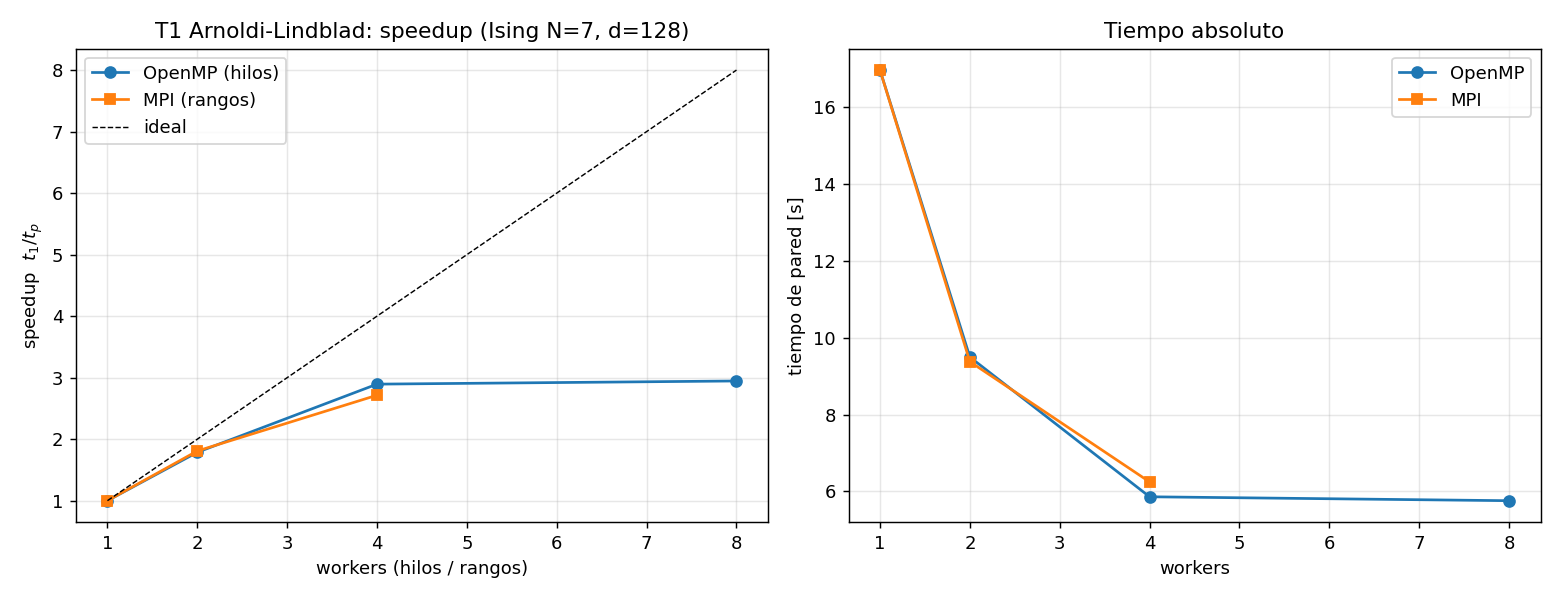
\includegraphics[width=\linewidth]{juan/T1/results/t1_scaling.png}\\
    {\scriptsize\textcolor{soft}{Escalado fuerte (Ising $N=7$, $d=128$).}}
  \end{column}
  \begin{column}{0.5\textwidth}
    \small
    \textbf{Computacional.}
    \begin{itemize}\small
      \item OpenMP $\,2.9\times\,$ / MPI $\,2.7\times\,$ (4 workers).
      \item \emph{Plateau} en los núcleos físicos: SpMV \emph{memory-bound}; el
        $\Lop$ está \cs{acoplado} $\Rightarrow$ comunicación \texttt{Allgatherv}.
    \end{itemize}
    \textbf{Validación / física.}
    \begin{itemize}\small
      \item Error en $\lambda$ lentos: $10^{-13}$–$10^{-5}$ vs denso.
      \item \emph{Faster-than-the-clock} hasta $8.8\times$ en SpMV.
      \item Da el $\lambda_2$ y el $a_2$ que \cs{determinan el cruce} de Mpemba.
    \end{itemize}
  \end{column}
  \end{columns}
\end{frame}

% ====================================================================
\divider{seb}{Sebastián}{3 · Evolución temporal (a): RK4 directo}

\begin{frame}{T2a — Método y discretización\Sb}
  \small
  \textbf{Framework.} Integrar $\dot\rho=\Lop[\rho]$ paso a paso desde una
  preparación $\rho_0$ y trazar $D_{HS}(\rho_t\|\rss)$.
  \medskip

  \textbf{Discretización: Runge--Kutta 4 (RK4)}, $\rho_{n+1}=\rho_n+\tfrac{\Delta t}{6}(k_1{+}2k_2{+}2k_3{+}k_4)$,
  con cada $k_i=\Lop[\,\cdot\,]$ \emph{matrix-free}
  $\;\Lop[V]=-i(HV{-}VH)+\sum_\mu(L_\mu V L_\mu^\dagger-\tfrac12\{L_\mu^\dagger L_\mu,V\})$.
  \begin{itemize}\small
    \item Orden global $\mathcal{O}(\Delta t^4)$; coste por paso $\mathcal{O}(N d^3)$
      (el \cs{producto de matrices} densas domina).
    \item \textbf{Paralelización: OpenMP.} Pasos con dependencia temporal estricta
      $\Rightarrow$ el paralelismo está \emph{dentro} del paso, en el \texttt{matmul}.
      Memoria compartida, sin halo $\Rightarrow$ OpenMP (no MPI).
  \end{itemize}
\end{frame}

\begin{frame}[fragile]{T2a — Núcleo: serial \textbar\ paralelo (OpenMP)\Sb}
  \begin{columns}[T]
  \begin{column}{0.48\textwidth}
  \centering\textbf{\small Serial}
\begin{lstlisting}[language=C++]
Mat matmul(A,B,d){
 Mat C(d*d);
 for(int i=0;i<d;++i)
  for(int k=0;k<d;++k){
   cd a=A[i*d+k];
   for(int j=0;j<d;++j)
    C[i*d+j]+=a*B[k*d+j];}
 return C;}
\end{lstlisting}
  \end{column}
  \begin{column}{0.52\textwidth}
  \centering\textbf{\small Paralelo}
\begin{lstlisting}[language=C++]
Mat matmul(A,B,d){
 Mat C(d*d);
 #pragma omp parallel for schedule(static)
 for(int i=0;i<d;++i)
  for(int k=0;k<d;++k){
   cd a=A[i*d+k];
   for(int j=0;j<d;++j)
    C[i*d+j]+=a*B[k*d+j];}
 return C;}
\end{lstlisting}
  \end{column}
  \end{columns}
  \vfill
  {\small Una sola \cs{\#pragma omp parallel for} reparte las filas $i$ entre hilos
  (independientes, sin condiciones de carrera). El \emph{mismo} binario, con distinto
  \texttt{OMP\_NUM\_THREADS}, da las curvas serie vs paralelo.}
\end{frame}

\begin{frame}{T2a — Resultados: computacional y físico\Sb}
  \begin{columns}[T]
  \begin{column}{0.5\textwidth}
    \centering
    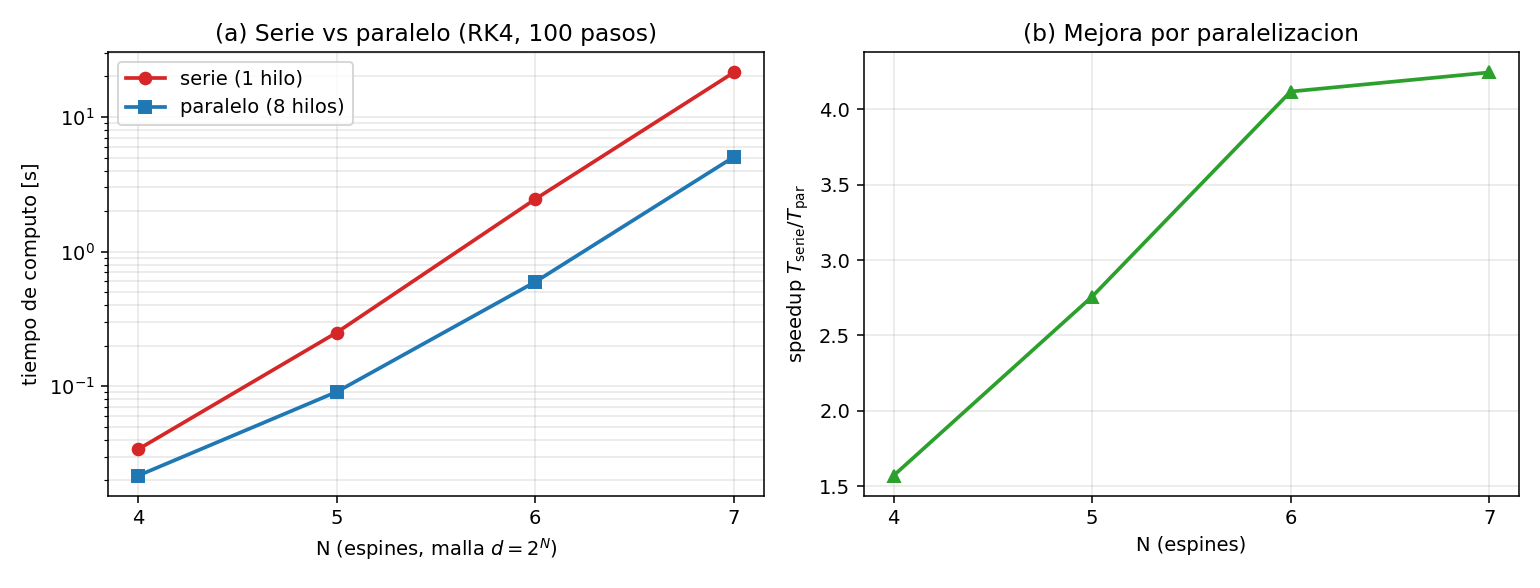
\includegraphics[width=\linewidth]{T2/a_integracion_directa/results/fig_t2a_serial_parallel.png}\\
    {\scriptsize\textcolor{soft}{Serie vs paralelo vs tamaño $N$: speedup $\to\!4\times$.}}
  \end{column}
  \begin{column}{0.5\textwidth}
    \centering
    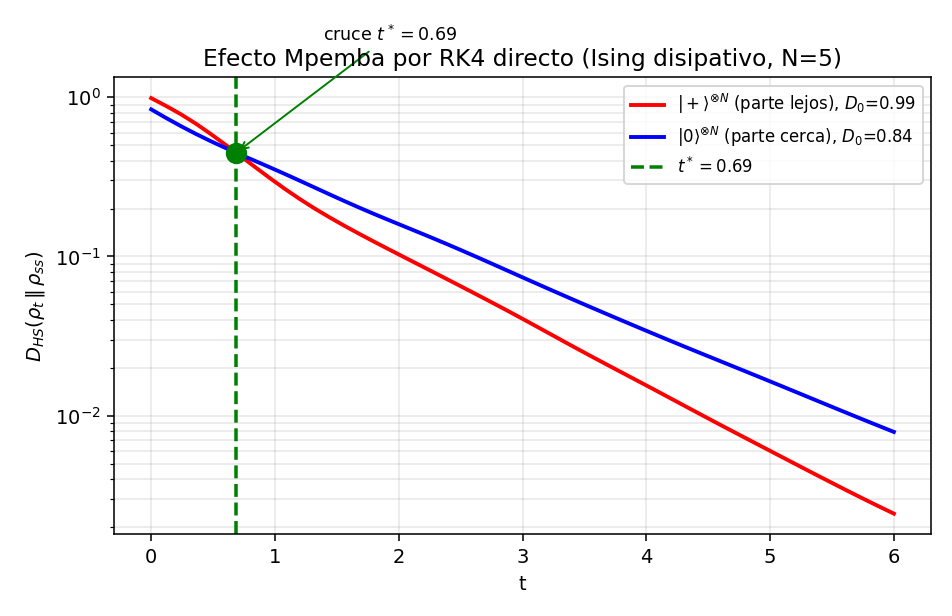
\includegraphics[width=\linewidth]{T2/a_integracion_directa/results/fig_t2a_mpemba.png}\\
    {\scriptsize\textcolor{soft}{\cs{Cruce de Mpemba} por RK4: $t^*\!\approx\!0.69$.}}
  \end{column}
  \end{columns}
  \vfill
  {\small RK4 validado a orden 4 ($\approx4.04$); speedup OpenMP sublineal
  (\emph{bandwidth-bound}). \cs{La curva que parte lejos adelanta a la cercana en $t^*$.}}
\end{frame}

% ====================================================================
\divider{seb}{Sebastián}{4 · Evolución temporal (b): Krylov}

\begin{frame}{T2b — Krylov: método y el resultado central\Sb}
  \small
  \textbf{Idea.} En vez de integrar paso a paso, aplicar la \cs{acción del
  exponencial} $\rho(t{+}\tau)=e^{\tau\Lop}[\rho]$ proyectando en un subespacio de
  Krylov $\mathcal{K}_m$ (Arnoldi) y exponenciando la matriz pequeña $m\times m$
  \cite{Sidje1998,AlMohyHigham2011}.
  \begin{columns}[T]
  \begin{column}{0.5\textwidth}
  \begin{itemize}\small
    \item \emph{Mismo hotspot} que RK4 (el \texttt{matmul} de $\Lop[\cdot]$)
      $\Rightarrow$ misma paralelización OpenMP, escalado equivalente.
    \item Ventaja: \cs{mucho menos trabajo} para igual precisión, y pasos $\tau$
      grandes (incondicionalmente estable).
  \end{itemize}
  \end{column}
  \begin{column}{0.5\textwidth}
    \centering
    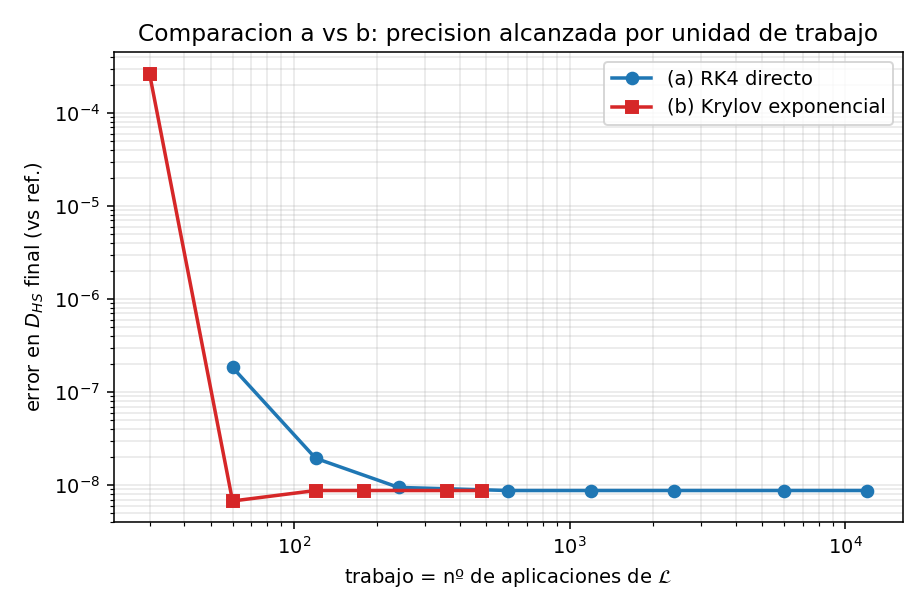
\includegraphics[width=0.92\linewidth]{T2/b_accion_exponencial/results/fig_t2b_method_compare.png}\\
    {\scriptsize\textcolor{soft}{A igual trabajo, Krylov $\sim25\times$ más preciso que RK4.}}
  \end{column}
  \end{columns}
\end{frame}

\begin{frame}{T2b — El cruce de Mpemba por Krylov\Sb}
  \begin{columns}[T]
  \begin{column}{0.55\textwidth}
    \centering
    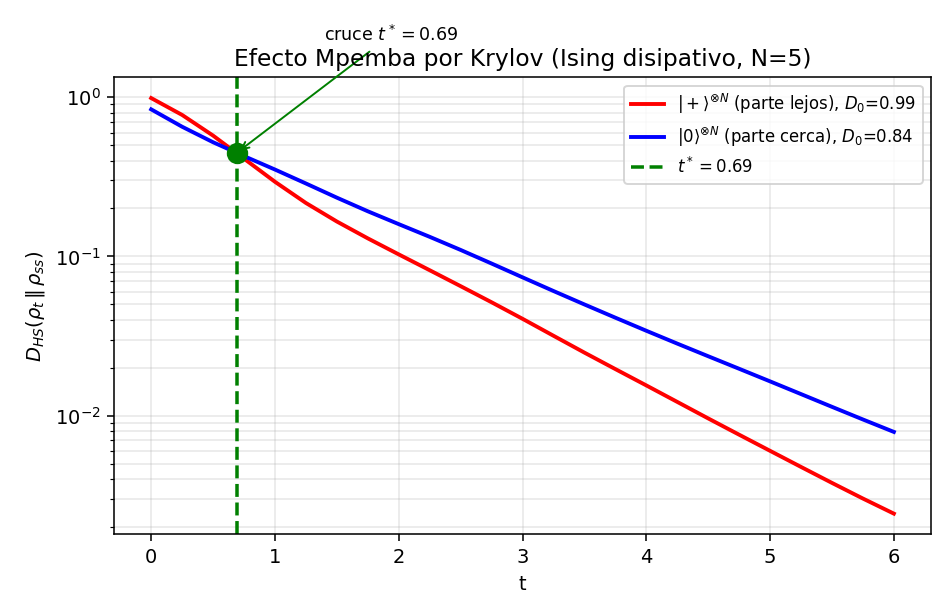
\includegraphics[width=0.9\linewidth]{T2/b_accion_exponencial/results/fig_t2b_mpemba.png}
  \end{column}
  \begin{column}{0.45\textwidth}
    \small
    \cs{Cruce en $t^*\!\approx\!0.69$}, idéntico al de RK4: el cruce es \emph{físico},
    no del integrador.
    \medskip

    Krylov reproduce exactamente la misma trayectoria (acuerdo a $10^{-10}$ en
    $D_{HS}$ final) con pasos de tiempo grandes.
  \end{column}
  \end{columns}
\end{frame}

% ====================================================================
\divider{seb}{Sebastián}{5 · Muchos cuerpos: trayectorias (MPI)}

\begin{frame}[fragile]{T3 — Trayectorias: método y núcleo serial \textbar\ paralelo\Sb}
  \small
  \textbf{Monte Carlo wavefunction} \cite{Daley2014,Johansson2013}: propagar $M$ estados
  \emph{puros} $\ket\psi\in\mathbb{C}^d$ (memoria $d$, no $d^2$) y promediar
  $\rho=\mathbb{E}[\dyad{\psi}{\psi}]$. \cs{Embarrassingly parallel}.
  \begin{columns}[T]
  \begin{column}{0.46\textwidth}
  \centering\textbf{\scriptsize Serial}
\begin{lstlisting}[language=C++]
for(int tr=0;tr<M;++tr){
 psi=ket0;
 for(paso) RK4_Heff+salto(psi);
 acc += |psi><psi|;
}
rho = acc / M;
\end{lstlisting}
  \end{column}
  \begin{column}{0.54\textwidth}
  \centering\textbf{\scriptsize Paralelo (MPI)}
\begin{lstlisting}[language=C++]
int my_M = M/size + ...;     // reparto
for(int tr=0;tr<my_M;++tr){
 ... acc_local += |psi><psi|;
}
MPI_Reduce(acc_local,acc,MPI_SUM,0);
if(rank==0) rho = acc / M;   // 1 sola colectiva
\end{lstlisting}
  \end{column}
  \end{columns}
  \vfill
  {\small Cada rango integra su lote \emph{sin comunicación}; una única
  \cs{MPI\_Reduce} promedia. Sin halo ni dependencias $\Rightarrow$ escalado casi ideal.}
\end{frame}

\begin{frame}{T3 — Resultados: computacional y físico\Sb}
  \begin{columns}[T]
  \begin{column}{0.5\textwidth}
    \centering
    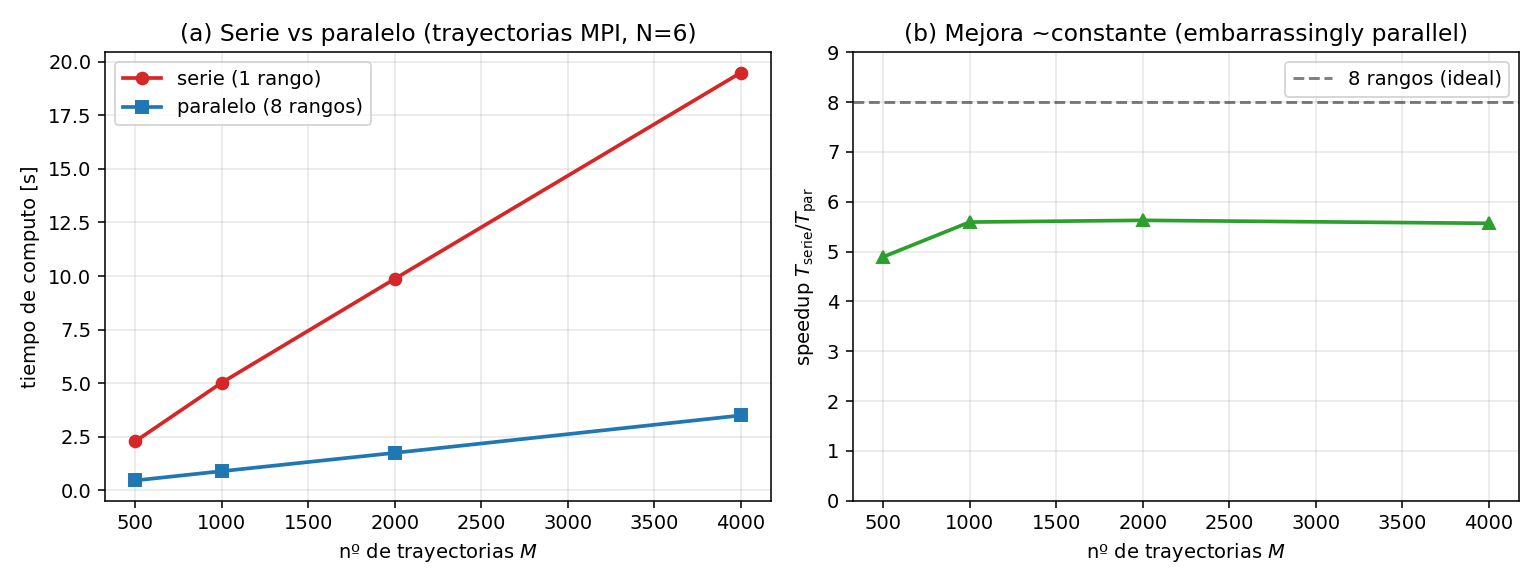
\includegraphics[width=\linewidth]{T3/integration/results/fig_t3_serial_parallel.png}\\
    {\scriptsize\textcolor{soft}{Serie vs paralelo vs $M$: speedup $\approx5.6\times$ \emph{constante}.}}
  \end{column}
  \begin{column}{0.5\textwidth}
    \centering
    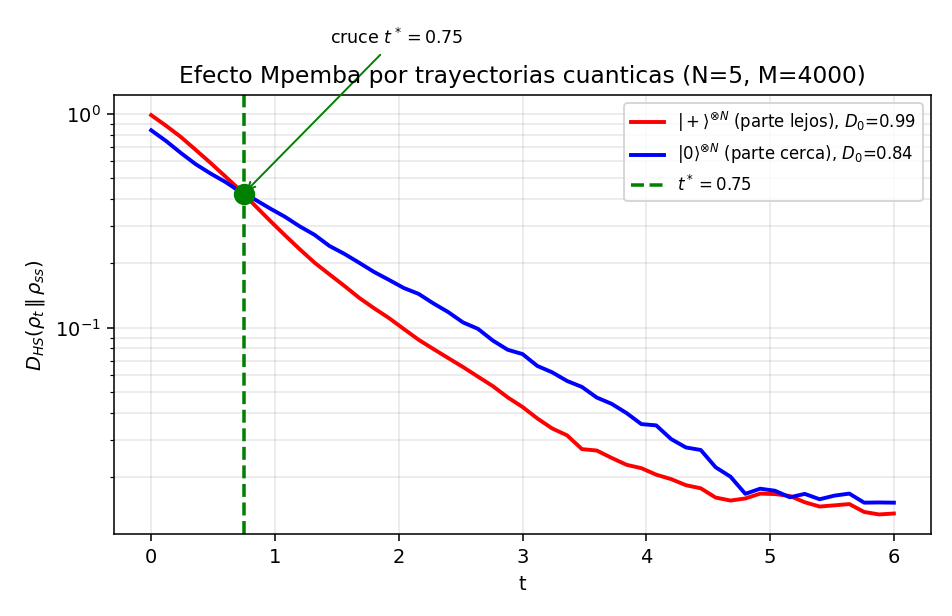
\includegraphics[width=\linewidth]{T3/integration/results/fig_t3_mpemba.png}\\
    {\scriptsize\textcolor{soft}{\cs{Cruce de Mpemba} por trayectorias: $t^*\!\approx\!0.75$.}}
  \end{column}
  \end{columns}
  \vfill
  {\small Convergencia estadística $M^{-1/2}$; el MPI escala \emph{casi ideal}
  (contraste con el OpenMP sublineal de T2): \cs{el patrón de cómputo dicta el paradigma}.}
\end{frame}

\begin{frame}{T3 — Aceleración en GPU (CUDA / T4)\Sb}
  \begin{columns}[T]
  \begin{column}{0.5\textwidth}
    \centering
    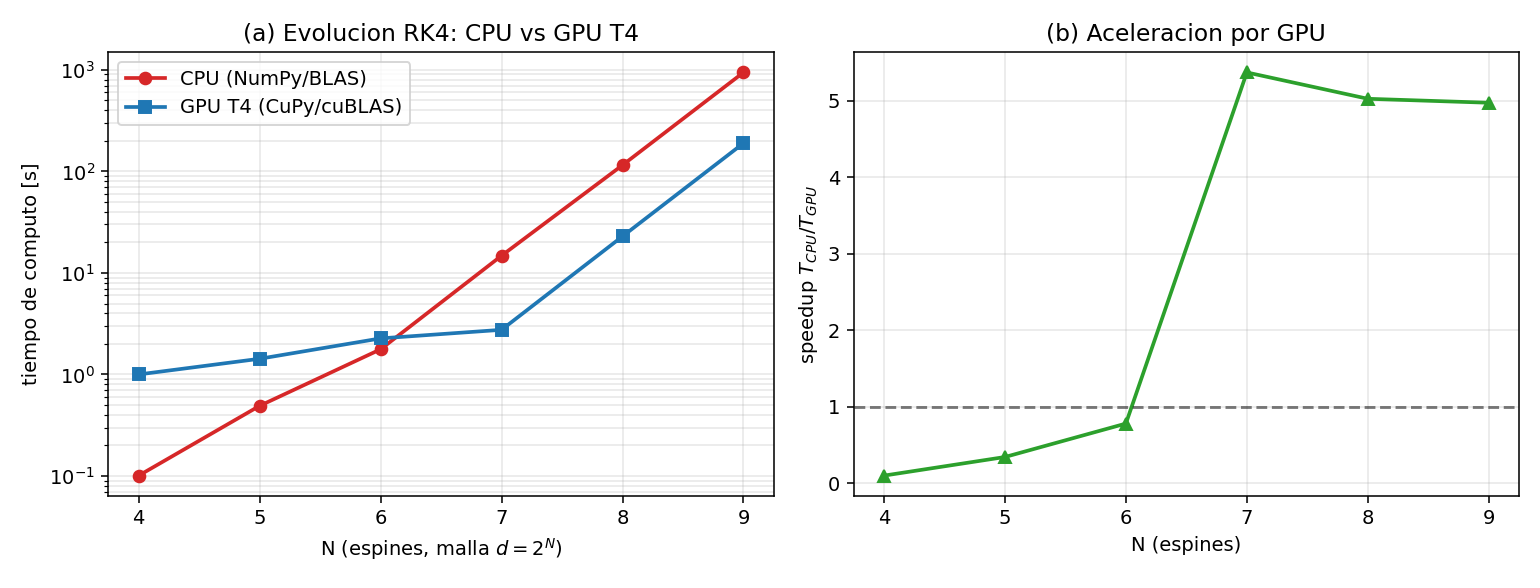
\includegraphics[width=\linewidth]{T2/cuda/results/fig_t2_cuda_evolution.png}\\
    {\scriptsize\textcolor{soft}{Evolución RK4: CPU vs GPU T4 (cuBLAS).}}
  \end{column}
  \begin{column}{0.5\textwidth}
    \small
    \textbf{Tercer escalón:} serie $\to$ OpenMP $\to$ \cs{CUDA T4}. El \texttt{matmul}
    denso $\to$ cuBLAS \texttt{zgemm}.
    \begin{itemize}\small
      \item GPU pierde a $d$ pequeño (overhead de kernels) y \cs{gana $\sim5\times$}
        a $N\!\ge\!7$ ($N{=}9$: 943\,s CPU $\to$ 190\,s GPU).
      \item GEMM hasta $250$ GFLOP/s ($d{=}2048$).
      \item Validación triple GPU $=$ CPU $=$ C++ ($D_{HS}\!\to\!0$).
    \end{itemize}
    {\scriptsize\textcolor{soft}{Notebook ejecutado + \texttt{resultados\_t2\_cuda.zip} en \texttt{T2/cuda/}.}}
  \end{column}
  \end{columns}
\end{frame}

% ====================================================================
\divider{juan}{Juan}{6 · Muchos cuerpos: redes tensoriales}

\begin{frame}{T3b — Redes tensoriales: método y discretización\J}
  \small
  \textbf{TEBD disipativo} \cite{Weimer2021,Orus2014}. La matriz densidad se escribe
  como un \cs{\emph{superket}} $|\rho\rangle\rangle$ (un MPS de dimensión física 4 por
  sitio) y se integra $\partial_t|\rho\rangle\rangle=\Lop|\rho\rangle\rangle$:
  \begin{itemize}\small
    \item \textbf{Trotter} de $e^{dt\,\Lop}$ en compuertas locales de 2 sitios.
    \item \textbf{Truncación} del rango de enlace a $\chi$ por SVD $\Rightarrow$ coste
      \cs{polinómico en $\chi$} (no exponencial en $N$).
    \item \textbf{Paralelización: hilos.} En una capa, los bonds \emph{pares} (o
      impares) son disjuntos $\Rightarrow$ sus SVD ($\mathcal{O}(\chi^3)$) son
      independientes. numpy \cs{libera el GIL} en la SVD/BLAS.
  \end{itemize}
\end{frame}

\begin{frame}[fragile]{T3b — Núcleo: serial \textbar\ paralelo (hilos)\J}
  \begin{columns}[T]
  \begin{column}{0.46\textwidth}
  \centering\textbf{\small Serial}
\begin{lstlisting}[language=Python]
# capa de Trotter
for k in bonds:        # disjuntos
    mps.apply_gate(
        k, gate, chi)  # SVD O(chi^3)
\end{lstlisting}
  \end{column}
  \begin{column}{0.54\textwidth}
  \centering\textbf{\small Paralelo (ThreadPool)}
\begin{lstlisting}[language=Python]
executor.map(
    lambda k: mps.apply_gate(k, gate, chi),
    bonds)             # SVD libera el GIL
# capas par / impar -> bonds independientes
\end{lstlisting}
  \end{column}
  \end{columns}
  \vfill
  {\small Paralelismo \cs{estructurado}: intermedio entre el SpMV acoplado (T1) y las
  trayectorias independientes (T3). Se mapea a MPI repartiendo segmentos de la cadena.}
\end{frame}

\begin{frame}{T3b — Implementación y resultados\J}
  \begin{columns}[T]
  \begin{column}{0.34\textwidth}
    \centering
    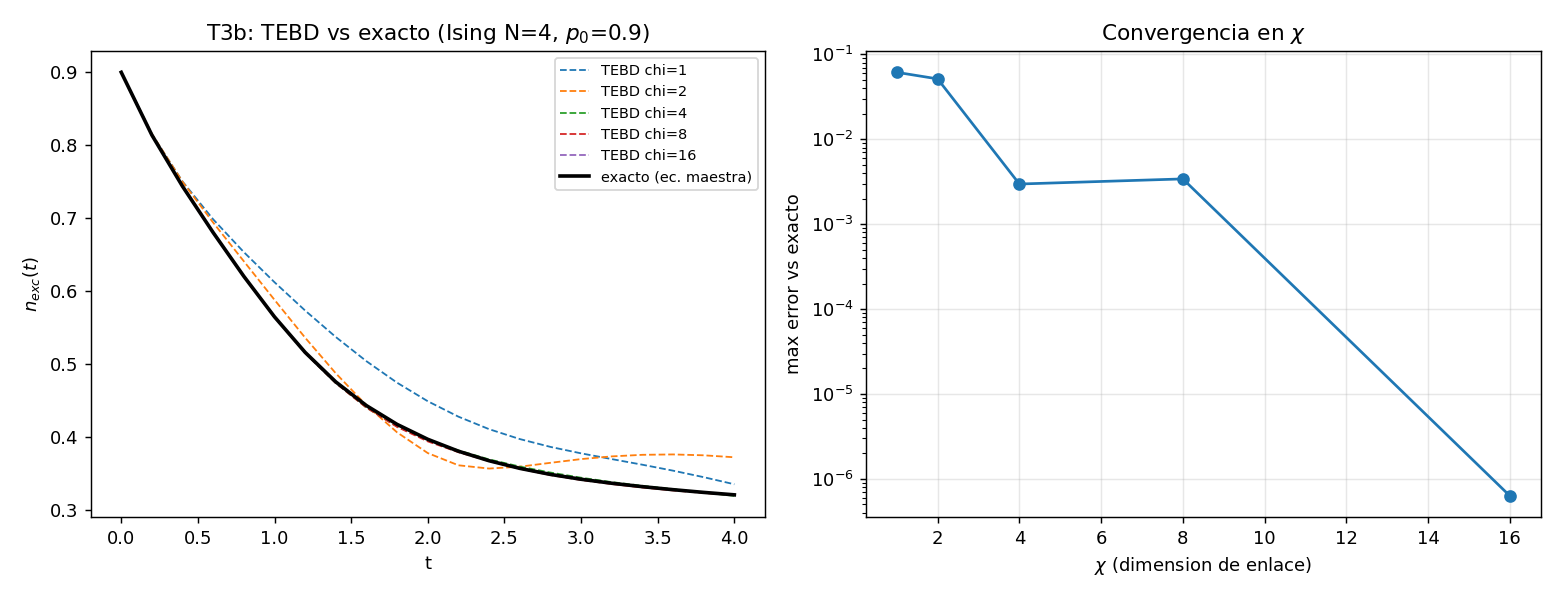
\includegraphics[width=\linewidth]{juan/T3/T3b_tensor_networks/results/t3b_validation.png}\\
    {\scriptsize\textcolor{soft}{Error $\to6\times10^{-7}$ al subir $\chi$.}}
  \end{column}
  \begin{column}{0.34\textwidth}
    \centering
    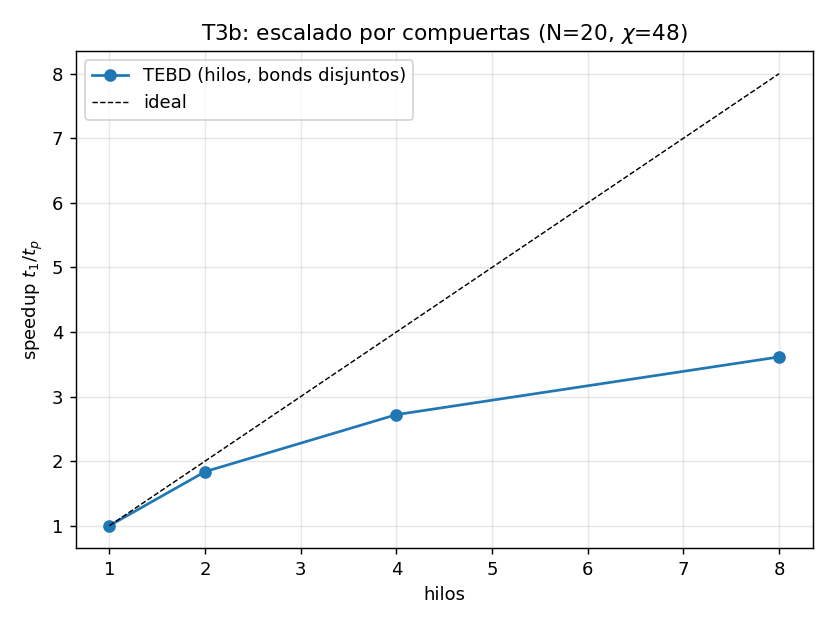
\includegraphics[width=\linewidth]{juan/T3/T3b_tensor_networks/results/t3b_scaling.png}\\
    {\scriptsize\textcolor{soft}{Hilos: $3.6\times$ (8).}}
  \end{column}
  \begin{column}{0.32\textwidth}
    \small
    \textbf{Alcance.}
    \begin{itemize}\small
      \item Validado vs exacto: error cae con $\chi$.
      \item \cs{$N=32$} ($4^{32}\!\approx\!10^{19}$), imposible en denso, en $\sim$3.6\,s.
    \end{itemize}
    {\scriptsize\textcolor{soft}{Las redes tensoriales abren el régimen de muchos cuerpos
    donde T1/T2 no llegan.}}
  \end{column}
  \end{columns}
\end{frame}

\begin{frame}{T3b — El cruce de Mpemba (redes tensoriales)\J}
  \begin{columns}[T]
  \begin{column}{0.55\textwidth}
    \centering
    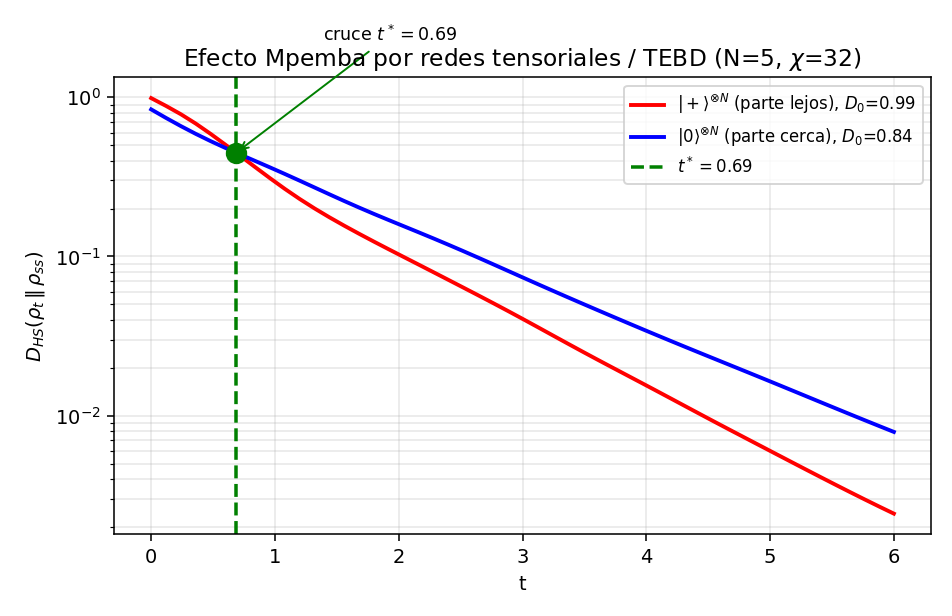
\includegraphics[width=0.92\linewidth]{juan/T3/T3b_tensor_networks/results/fig_t3b_mpemba.png}
  \end{column}
  \begin{column}{0.45\textwidth}
    \small
    También TEBD reproduce el efecto: $\ket{+}^{\otimes N}$ (parte lejos)
    \textbf{adelanta} a $\ket{0}^{\otimes N}$ en \cs{$t^*\!\approx\!0.69$}.
    \medskip

    Idéntico a RK4/Krylov (a $\chi$ grande TEBD es exacto): \cs{el cruce es físico},
    y aquí se obtiene con el método que escala a muchos cuerpos.
    \medskip

    {\scriptsize\textcolor{soft}{Los \textbf{cuatro} métodos de evolución
    (RK4, Krylov, trayectorias, redes tensoriales) dan el mismo $t^*$.}}
  \end{column}
  \end{columns}
\end{frame}

% ====================================================================
\divider{juan}{Juan}{7 · Conclusiones generales}

\begin{frame}{Conclusiones — HPC y física\J}
  \begin{columns}[T]
  \begin{column}{0.5\textwidth}
    \cj{HPC: el patrón de cómputo dicta el paradigma}
    \begin{itemize}\small
      \item \textbf{T1} SpMV \emph{acoplado} (OpenMP/MPI $\sim2.9\times$).
      \item \textbf{T3b} \emph{estructurado} (hilos $\sim3.6\times$).
      \item \textbf{T3} \emph{embarrassingly parallel} (MPI $\sim5.6\times$, casi ideal).
      \item \textbf{T2} evolución densa $\to$ \cs{GPU} (cuBLAS $\sim5\times$).
    \end{itemize}
    {\scriptsize Espectro de escalabilidad: acoplado $<$ estructurado $<$ independiente.}
  \end{column}
  \begin{column}{0.5\textwidth}
    \cs{Física: el efecto Mpemba cuántico}
    \begin{itemize}\small
      \item Origen \emph{geométrico-espectral}: no-normalidad de $\Lop$ + criterio
        $a_2=0$ \cite{Carollo2021}.
      \item \cs{Cruce reproducido por los 4 métodos} de evolución (RK4, Krylov,
        trayectorias, redes tensoriales; $t^*\!\approx\!0.69$–$0.75$), validado de forma cruzada.
      \item Escalable a muchos cuerpos vía trayectorias y redes tensoriales.
    \end{itemize}
  \end{column}
  \end{columns}
\end{frame}

% ====================================================================
\divider{seb}{Sebastián}{8 · Relevancia en el efecto macro/meso}

\begin{frame}{Del cuántico al mesoscópico y macroscópico\Sb}
  \begin{columns}[T]
  \begin{column}{0.5\textwidth}
    \small
    \textbf{La firma es universal.} El mismo mecanismo —\cs{geometría espectral de
    la relajación}— explica el cruce en cascadas clásicas, coloides y sistemas
    cuánticos \cite{LuRaz2017,Kumar2022,Teza2026}.
    \medskip

    \textbf{Lo que devuelve el enfoque cuántico:}
    \begin{itemize}\small
      \item Un \emph{criterio operacional} ($a_2=0$) y herramientas HPC para
        \emph{predecir} y \emph{diseñar} el efecto.
      \item Aplicaciones: \cs{termometría cuántica} y enfriamiento acelerado
        \cite{Manikandan2021,Ivander2023}.
    \end{itemize}
  \end{column}
  \begin{column}{0.5\textwidth}
    \centering
    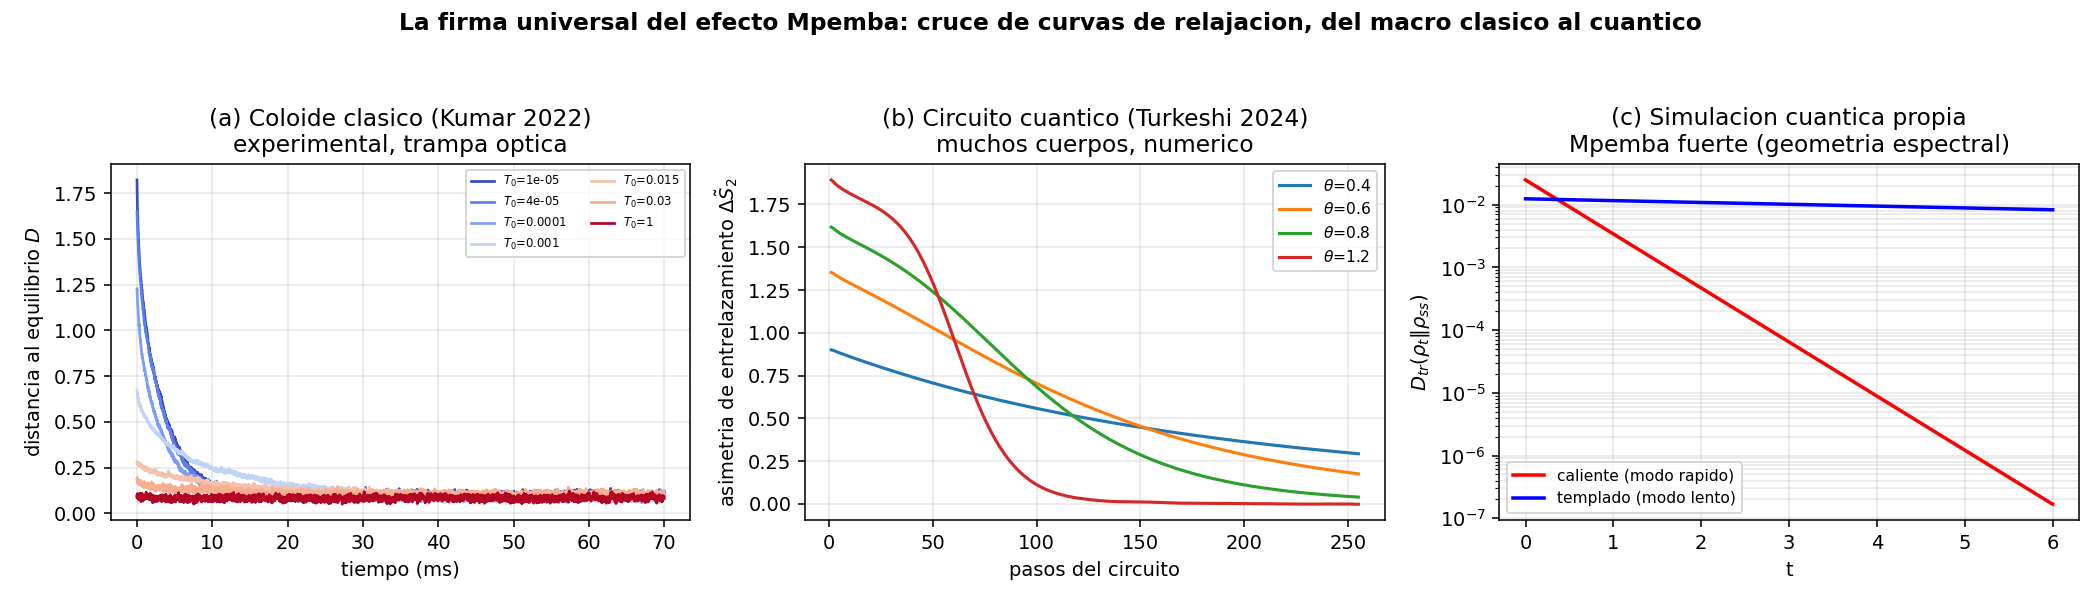
\includegraphics[width=\linewidth]{macro/results/fig_macro_universal.png}\\
    {\scriptsize\textcolor{soft}{La firma universal del cruce: del macro al cuántico.}}
  \end{column}
  \end{columns}
\end{frame}

% ---------------------------------------------------------------- REFS
\begin{frame}[allowframebreaks]{Referencias}
  \scriptsize
  \bibliographystyle{abbrv}
  \bibliography{../context/doc/referencias}
\end{frame}

\begin{frame}[plain]
  \vfill\centering
  {\Large\bfseries ¡Gracias!}\\[6pt]
  {\small \cj{Juan} \;\textbar\; \cs{Sebastián} \quad ---\quad Efecto Mpemba cuántico en HPC}
  \vfill
\end{frame}

\end{document}
